% TikZ figure: PWLC value function for a two-state POMDP
% Illustrates how the value function is piecewise linear and convex
% over the one-dimensional belief space b = Pr(s1)

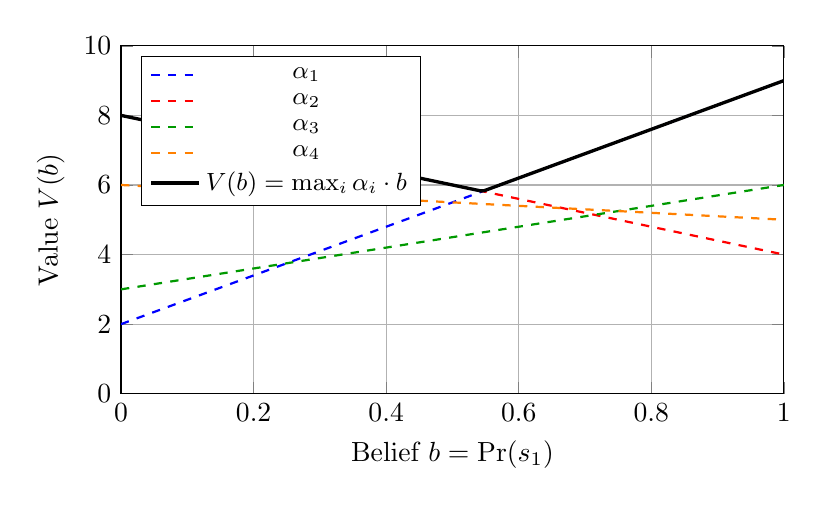
\begin{tikzpicture}[scale=1.0]
  \begin{axis}[
    width=10cm,
    height=6cm,
    xlabel={Belief $b = \Pr(s_1)$},
    ylabel={Value $V(b)$},
    xmin=0, xmax=1,
    ymin=0, ymax=10,
    xtick={0, 0.2, 0.4, 0.6, 0.8, 1.0},
    ytick={0, 2, 4, 6, 8, 10},
    grid=both,
    grid style={line width=0.2pt, draw=gray!30},
    major grid style={line width=0.4pt, draw=gray!60},
    legend pos=north west,
    legend style={font=\small},
  ]

    % Individual alpha vectors (linear functions of b)
    \addplot[blue,   dashed, thick, domain=0:1] {2 + 7*x}   node[right, pos=1] {};
    \addplot[red,    dashed, thick, domain=0:1] {8 - 4*x}   node[right, pos=1] {};
    \addplot[green!60!black, dashed, thick, domain=0:1] {3 + 3*x} node[right, pos=1] {};
    \addplot[orange, dashed, thick, domain=0:1] {6 - 1*x}   node[right, pos=1] {};

    % The PWLC envelope (upper envelope = value function)
    \addplot[black, very thick, domain=0:1, samples=200] {max(max(2+7*x, 8-4*x), max(3+3*x, 6-1*x))};

    \addlegendentry{$\alpha_1$}
    \addlegendentry{$\alpha_2$}
    \addlegendentry{$\alpha_3$}
    \addlegendentry{$\alpha_4$}
    \addlegendentry{$V(b) = \max_i \alpha_i \cdot b$}

  \end{axis}
\end{tikzpicture}
